\documentclass{beamer}

\mode<presentation> {
\usetheme{CambridgeUS}
\usecolortheme{seagull}
\usefonttheme{default}
}

\usepackage{graphicx}
\usepackage{booktabs}
\usepackage{ragged2e}
\usepackage{minted}
\usepackage{lipsum}
\usepackage[export]{adjustbox}

%----------------------------------------------------------------------------------------
%	My Customized Settings
%----------------------------------------------------------------------------------------

\definecolor{UniBlue}{RGB}{83,121,170}
\definecolor{DarkGray}{RGB}{90,90,90}
\definecolor{LightGray}{RGB}{150,150,150}
\definecolor{TextGreen}{RGB}{115,155,15}
\definecolor{Ocean}{RGB}{23,142,189}
\definecolor{BG}{RGB}{215,215,215}


\setbeamercolor{normal}{fg=DarkGray}
\setbeamercolor{title}{fg=UniBlue}
\setbeamercolor{frametitle}{fg=UniBlue}
\setbeamercolor{structure}{fg=UniBlue}
\setbeamercolor{normal text}{fg=DarkGray,bg=white}
\setbeamercolor{section number projected}{bg=UniBlue,fg=white}

\setbeamertemplate{itemize item}{\scriptsize\raise1.25pt\hbox{\donotcoloroutermaths$\blacktriangleright$}}
\setbeamertemplate{itemize subitem}{\tiny\raise1.5pt\hbox{\donotcoloroutermaths$\bullet$}}
\setbeamertemplate{itemize subsubitem}{\tiny\raise1.5pt\hbox{\donotcoloroutermaths$\blacksqaure$}}
\setbeamercolor{itemize item}{fg=darkred}
\setbeamercolor{itemize subitem}{fg=TextGreen}
\setbeamercolor{itemize subbody}{fg=LightGray}

\setbeamertemplate{enumerate subitem}{\insertenumlabel.\insertsubenumlabel}
\setbeamertemplate{enumerate subsubitem}{\insertenumlabel.\insertsubenumlabel.\insertsubsubenumlabel}
\setbeamertemplate{enumerate mini template}{\insertenumlabel}

\setbeamertemplate{navigation symbols}{}

\newcommand\VeryLargeFont{\fontsize{30}{15}\selectfont}
\newcommand\LargeFont{\fontsize{15}{15}\selectfont}
\newcommand\TinyFont{\fontsize{6}{6}\selectfont}

\setbeamertemplate{frametitle} {
  \nointerlineskip
  \begin{beamercolorbox}[sep=0.15cm,ht=1.3em,wd=\paperwidth]{frametitle}
    \vbox{}\vskip-2ex
    \strut\insertframetitle\strut
    \vskip-0.8ex
  \end{beamercolorbox}
}

\defbeamertemplate*{title page}{customized}[1][] {
  \centering
  \bigskip
  \bigskip
  \bigskip
  \usebeamercolor[fg]{title}\insertsubtitle\par
  \usebeamerfont{title}\inserttitle\par
  \usebeamerfont{subtitle}
  \bigskip
  \usebeamercolor[fg]{normal}
  \usebeamerfont{author}\insertauthor\par
  \usebeamerfont{institute}\insertinstitute\par
  \usebeamerfont{date}\insertdate\par
  \bigskip
  \bigskip
  \bigskip
  \bigskip
  \bigskip
  \usebeamercolor[fg]{titlegraphic}\inserttitlegraphic
}

%----------------------------------------------------------------------------------------
%	TITLE PAGE
%----------------------------------------------------------------------------------------
\title[Operating Systems of the IoT]{An Introduction to Operating Systems of the IoT}
\author{Elahe Jalalpoor \& Parham Alvani}
\institute[AUT] {
  Amirkabir University of Technology \\
  \medskip
  {\small\tt }
}
\date{Jun 18, 2015}
\titlegraphic{\hspace*{5cm}
\includegraphics[width=2cm]{figs/aut_logo.jpeg}}

\begin{document}

\begin{frame}
\titlepage
\end{frame}

%----------------------------------------------------------------------------------------
%	PRESENTATION SLIDES
%----------------------------------------------------------------------------------------

%------------------------------------------------
\section{}
\subsection{}

%------------------------------------------------
\begin{frame}
	\begin{columns}
		\begin{column}{10cm}
			\vspace{2cm}
			\begin{block}{
				\centering\textcolor{darkred}{What is the IoT...}}
				\justifying
				The Internet of Things (IoT) is a scenario in which objects, animals or people are provided with unique identifiers and the ability to transfer data over a network without requiring human-to-human or human-to-computer interaction.\\
			\end{block}
		\end{column}
	\end{columns}
	\vspace{.75cm}
	\hspace*{8.5cm}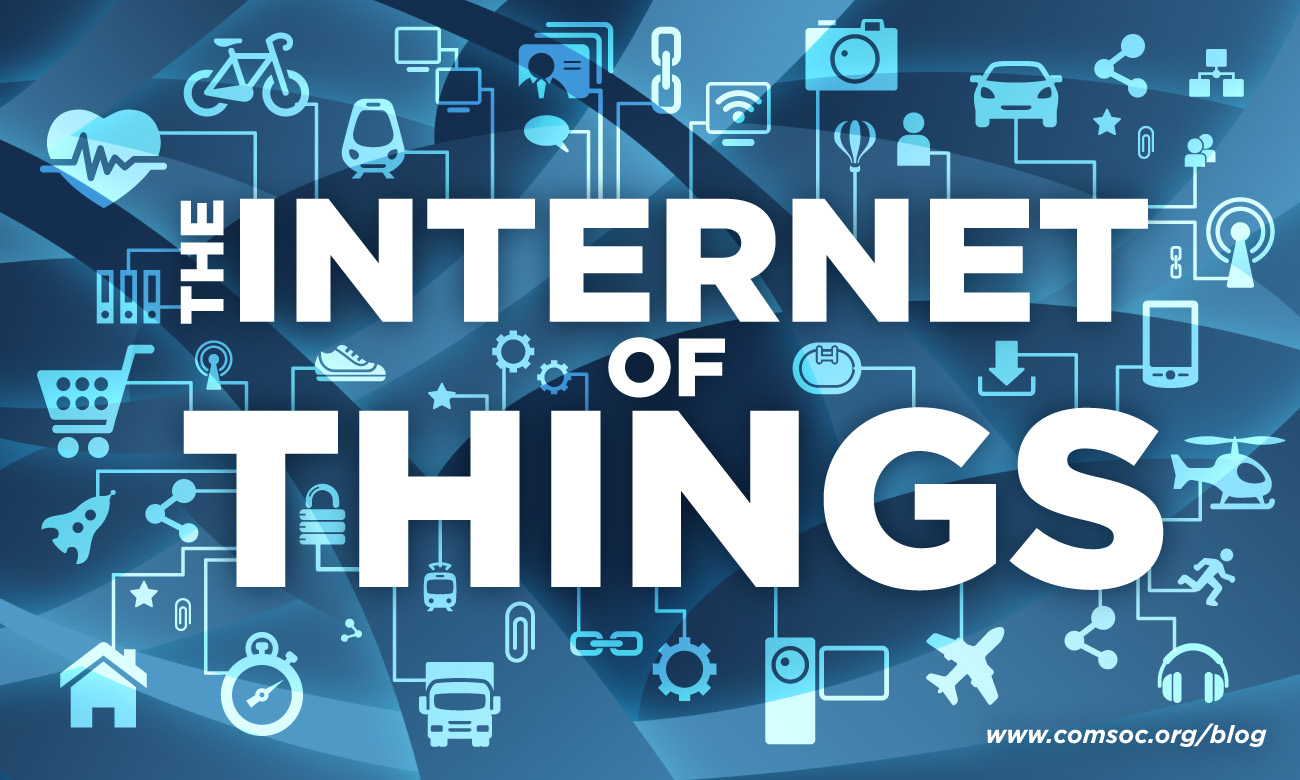
\includegraphics[width=3cm]{figs/Internet-of-Things-1.jpg}
\end{frame}

%------------------------------------------------
\begin{frame}
	\frametitle{Open Source Operating Systems for the IoT}
	\begin{columns}[c]
		\begin{column}{30cm}
			\vspace{.1cm}
			\begin{itemize}
				\justifying
				\item FreeRTOS
				\item Riot
				\item Contiki
				\item TinyOS
				\item OpenWSN
				\item Embedded Linux
			\end{itemize}
		\end{column}
	\end{columns}
	\vspace{.5cm}
	\hspace*{5.5cm} 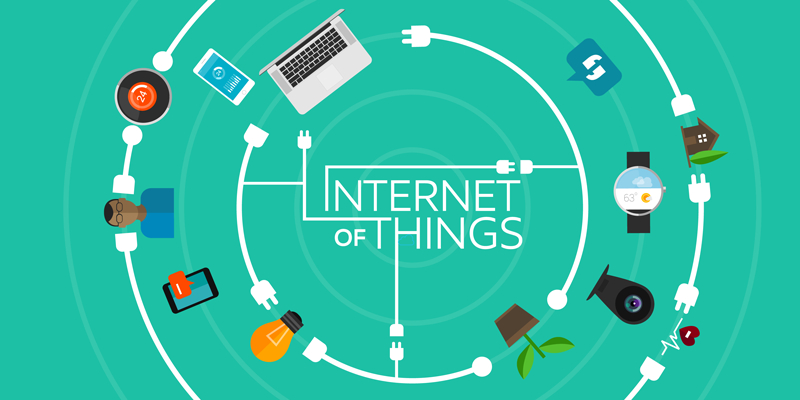
\includegraphics[width=5cm]{figs/Internet-of-Things-2.jpg}
\end{frame}

%------------------------------------------------
\begin{frame}
	\frametitle{FreeRTOS}
	\begin{columns}[c]
		\begin{column}{30cm}
			\vspace{.1cm}
			\begin{itemize}
				\justifying
				\item FreeRTOS is designed to be small and simple.
			\end{itemize}
		\end{column}
	\end{columns}
	\vspace{.5cm}
	\hspace*{5.5cm} 
\includegraphics[width=5cm]{figs/freertos-logo.jpg}	
\end{frame}

%------------------------------------------------
\begin{frame}
	\vspace{1cm}
	\begin{Huge}
		\begin{center}
			\usebeamercolor[fg]{title}Questions?
		\end{center}
	\end{Huge}
\end{frame}

\end{document} 
